% 2009 年重庆卷理科第 19 题：四棱锥 S-ABCD，E 为 BS 中点。
% 来源 PDF：普通高考/2009/2009重庆理.pdf，SHA-256 6a815fa472e380a3f1143e8cdd93712e142309acb7a95176783499406a8e15f1。
% 原页：第 2 页（A3 三栏）第 1 栏上部，书页码 504。
% 重绘依据：由题设取 D(0,0,0)、C(√6,0,0)、A(0,1,0)、B(√6,2,0)、S(√6/3,0,2/√3)。
%   投影取 (x,y,z) -> (x+0.35y, -1.2z+0.25y)，使 S 在下方、B 在上方，与原页视角一致。
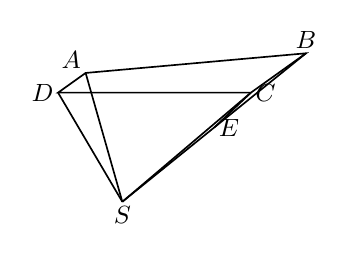
\begin{tikzpicture}[semithick, every node/.style={inner sep=1.4pt, font=\small}]
  \coordinate (D) at (0.000,0.000);
  \coordinate (C) at (2.449,0.000);
  \coordinate (A) at (0.350,0.250);
  \coordinate (B) at (3.149,0.500);
  \coordinate (S) at (0.816,-1.386);
  \coordinate (E) at (1.983,-0.443);

  % 底面
  \draw (A) -- (B) -- (C) -- (D) -- cycle;
  % 侧棱
  \draw (S) -- (D);
  \draw (S) -- (C);
  \draw (S) -- (A);
  \draw (S) -- (B);
  % CE
  \draw (C) -- (E);

  % 标注
  \node[left] at (D) {$D$};
  \node[right] at (C) {$C$};
  \node[above left] at (A) {$A$};
  \node[above] at (B) {$B$};
  \node[below] at (S) {$S$};
  \node[right] at (E) {$E$};
\end{tikzpicture}
